\documentclass[12p]{article}
\usepackage{tikz}
\usetikzlibrary{arrows,automata}
\usepackage{pgf}
\begin{document}
practica
\section{ejercicio 1}
Cosas que sabes del automata del ejercicio 3
la cadena 1001 pertence al lenguaje y por esto $ \delta(q_0 , 1001) = q _ 3$ , luego si llegara un 1 entonces el numero de (10)'s y (01)'s no cambiaria
pero nota que la cadena 01110 tambien pertenece al lenguaje y por lo tanto $\delta(q_0 , 01110) \in q_3 $ , pero en este caso si llegara un 1 \\
entonces el numero de (10)'s y (01)'s ya no seria el mismo y entonces se tendria que mover de estado,pero si llegara un cero entonces si seguiria
teniendo el mismo numero de (01)'s y (10)'s y lo mismo para el caso de arriba . Osea si llegara un 0 en el caso de arriba entonces
ya no tendrian el mismo numero de (10)'s y (01)'s.
Ahora para hacerlo mas sencillo vamos a reducir el problema para construir un automata que reconozca el lenguaje donde las subcadenas de 01 y 10
aparezcan el mismo numero de veces pero que comiencen con 1.
algunas cadenas que estan en el lenguaje son 1001 , 11, $\epsilon$ , 10001 , 1000100010001 , tambien 1001 101.
el lenguaje anterior tambien podria ser descrito como las cadenas que comienzan con 1 y terminan con 1 y tienen un numero par de 1's
debe haber un estado que especifique que hay un numero par de 1's
una vez que tenemos un automata que puede reconocer el lenguaje donde el numero de unos es par este tiene que ser extendido para
que cumpla la condicion de que las cadenas comiencen con 1 y
terminen con 1


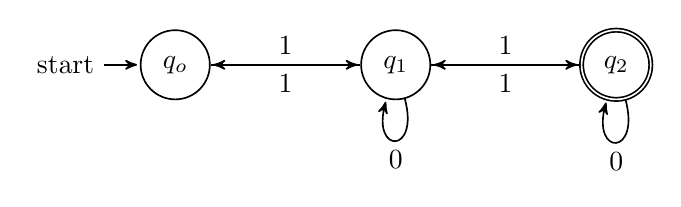
\begin{tikzpicture}[->,>=stealth',shorten >= 1pt,
  auto,node distance = 2.8cm,semithick ]
  \node[initial,state] (A) {$q_o$};
  \node[state] (B) [right of=A]{$q_1$};
  \node[state,accepting] (C) [right of=B]{$q _ 2$};
  \path
  (A) edge node {1} (B)
  (B) edge [loop below] node {0} (B)
  edge node {1} (C)
  edge node {1} (A)
  (C) edge [loop below] node {0} (C)
  edge node {1} (B);
\end{tikzpicture}
\end{document}